\documentclass{beamer}
\usepackage[utf8]{inputenc}

\usetheme{Madrid}
\usecolortheme{default}
\usepackage{amsmath,amssymb,amsfonts,amsthm}
\usepackage{txfonts}
\usepackage{tkz-euclide}
\usepackage{listings}
\usepackage{adjustbox}
\usepackage{array}
\usepackage{tabularx}
\usepackage{gvv}
\usepackage{lmodern}
\usepackage{circuitikz}
\usepackage{tikz}
\usepackage{graphicx}
\usepackage{multicol}

\setbeamertemplate{page number in head/foot}[totalframenumber]

\usepackage{tcolorbox}
\tcbuselibrary{minted,breakable,xparse,skins}



\definecolor{bg}{gray}{0.95}
\DeclareTCBListing{mintedbox}{O{}m!O{}}{%
  breakable=true,
  listing engine=minted,
  listing only,
  minted language=#2,
  minted style=default,
  minted options={%
    linenos,
    gobble=0,
    breaklines=true,
    breakafter=,,
    fontsize=\small,
    numbersep=8pt,
    #1},
  boxsep=0pt,
  left skip=0pt,
  right skip=0pt,
  left=25pt,
  right=0pt,
  top=3pt,
  bottom=3pt,
  arc=5pt,
  leftrule=0pt,
  rightrule=0pt,
  bottomrule=2pt,
  toprule=2pt,
  colback=bg,
  colframe=orange!70,
  enhanced,
  overlay={%
    \begin{tcbclipinterior}
    \fill[orange!20!white] (frame.south west) rectangle ([xshift=20pt]frame.north west);
    \end{tcbclipinterior}},
  #3,
}
\lstset{
    language=C,
    basicstyle=\ttfamily\small,
    keywordstyle=\color{blue},
    stringstyle=\color{orange},
    commentstyle=\color{green!60!black},
    numbers=left,
    numberstyle=\tiny\color{gray},
    breaklines=true,
    showstringspaces=false,
}
%------------------------------------------------------------
%This block of code defines the information to appear in the
%Title page
\title %optional
{4.13.34}
\date{September 30,2025}


\author 
{Jnanesh Sathisha karmar - EE25BTECH11029}



\begin{document}



\frame{\titlepage}
\begin{frame}{Question}The equations to a pair of opposite sides of parallogram are $x^2 - 5x + 6 = 0$ and $y^2 - 6y + 5 = 0$, the equations to its diagonals are
\begin{enumerate}
\begin{multicols}{2}
    \item $x+4y=13,y=4x-7$
    \item $4x+y=13,y=4x-7$
    \item $4x+y=13,4y=x-7$
    \item $y-4x=13,y+4x=7$
\end{multicols}
\end{enumerate}


\end{frame}

\begin{frame}{Theoretical Solution}
We can solve this problem by treating a pair of parallel lines as a degenerate conic section and finding where a line (the diagonal) intersects it. The general equation for a conic is given by $g(\vec{x}) = \vec{x}^\intercal \myvec{V} \vec{x} + 2\vec{u}^\intercal \vec{x} + f = 0$, and a parametric line is given by $\vec{x} = \vec{h} + \kappa\vec{m}$. The intersection points are found using the formula:
\noindent
\begin{align}
\kappa_{1,2} = \frac{-\vec{m}^{\top} \brak{\myvec{V}\vec{h} + \vec{u}} \pm \sqrt{\brak{\vec{m}^{\top} \brak{\myvec{V}\vec{h} + \vec{u}}}^2 - \brak{\vec{m}^{\top} \myvec{V} \vec{m}} g(\vec{h})}}{\vec{m}^{\top} \myvec{V} \vec{m}}
\end{align}

\end{frame}
\begin{frame}{Theoretical Solution}
Let's represent the pair of vertical lines $x^2 - (x_1+x_2)x + x_1x_2 = 0$ as our conic section.
\begin{align}
    \vec{V} &= \myvec{1&0\\0&0}, \quad 
    \vec{u} = \myvec{-\frac{x_1+x_2}{2}\\0}\ 
    f = x_1x_2
\end{align}
The diagonal is a line starting from the parallelogram's center $\vec{h}$ with a direction vector $\vec{m}$.
\begin{align}
    \vec{h} = \myvec{\frac{x_1+x_2}{2} \\ \frac{y_1+y_2}{2} },\ 
    \vec{m} = \myvec{ x_2-x_1 \\ y_2-y_1 }
\end{align}
\end{frame}

\begin{frame}{Theoretical Solution}
First, we evaluate the term $\vec{V}\vec{h} + \vec{u}$:
\vspace{0.2cm}
\begin{align}
    \vec{V}\vec{h} + \vec{u} = \myvec{ 1 & 0 \\ 0 & 0 } \myvec{ \frac{x_1+x_2}{2} \\ \frac{y_1+y_2}{2} } + \myvec{ -\frac{x_1+x_2}{2} \\ 0 } = \myvec{\frac{x_1+x_2}{2} \\ 0 } - \myvec{\frac{x_1+x_2}{2} \\ 0 } = \vec{0}
\end{align}
Since $\vec{V}\vec{h} + \vec{u} = \vec{0}$, the formula for $\kappa$ simplifies dramatically:
\vspace{0.2cm}
\noindent
\begin{align}
    \kappa_{1,2} = \frac{\pm \sqrt{-(\vec{m}^{\top} \myvec{V} \vec{m}) g(\vec{h})}}{\vec{m}^{\top} \myvec{V} \vec{m}}
\end{align}
\end{frame}
\begin{frame}{Theoretical Solution}
Next, we evaluate the remaining terms in the general case:
\begin{align}
    \vec{m}^{\top} \myvec{V} \vec{m} &= (x_2-x_1)^2 \\
    g(\vec{h}) &= \brak{\frac{x_1+x_2}{2}}^2 - (x_1+x_2)\brak{\frac{x_1+x_2}{2}} + x_1x_2 = -\frac{(x_2-x_1)^2}{4}
\end{align}
Substituting these back into the simplified formula for $\kappa$:
\vspace{0.2cm}
\noindent
\begin{align}
    \kappa_{1,2} = \frac{\pm \sqrt{-(x_2-x_1)^2 \brak{-\frac{(x_2-x_1)^2}{4}}}}{(x_2-x_1)^2} = \frac{\pm \sqrt{\frac{(x_2-x_1)^4}{4}}}{(x_2-x_1)^2} = \frac{\pm \frac{(x_2-x_1)^2}{2}}{(x_2-x_1)^2} = \pm \frac{1}{2}
\end{align}
This shows that the vertices are located at $\kappa = \pm 1/2$ from the center along the direction vector $\vec{m}$.
\end{frame}
\begin{frame}{Theoretical Solution}
\textbf{Applying to the specific problem:} \\
From $x^2 - 5x + 6 = 0$, we have $x_1=2, x_2=3$. \\
From $y^2 - 6y + 5 = 0$, we have $y_1=1, y_2=5$.

\noindent
The center point $\vec{h}$ and diagonal direction vectors $\vec{m}_1, \vec{m}_2$ are:
\vspace{0.2cm}
\begin{align}
    \vec{h} = \myvec{ 2.5 \\ 3 }, \ 
    \vec{m}_1 = \myvec{ 3-2 \\ 5-1 } = \myvec{ 1 \\ 4 }, \ 
    \vec{m}_2 = \myvec{ 2-3 \\ 5-1 } = \myvec{ -1 \\ 4 }
\end{align}
The vertices are $\vec{v} = \vec{h} \pm \frac{1}{2}\vec{m}$.

\noindent
\textbf{Diagonal 1 (using $\vec{m}_1$):}
\vspace{0.2cm}
\begin{align*}
    \vec{v}_C = \myvec{ 2.5 \\ 3 } + \frac{1}{2}\myvec{ 1 \\ 4 } = \myvec{ 3 \\ 5 } \  \text{and} \ 
    \vec{v}_A = \myvec{ 2.5 \\ 3 } - \frac{1}{2}\myvec{ 1 \\ 4 } = \myvec{ 2 \\ 1 }
\end{align*}
The line passing through $\vec{A}\brak{2,1}$ and $\vec{C}\brak{3,5}$ is $y-1 = 4\brak{x-2} \implies \boldsymbol{y = 4x - 7}$.
\end{frame}
\begin{frame}{Theoretical Solution}
    \textbf{Diagonal 2 (using $\vec{m}_2$):}
\begin{align*}
    \vec{v}_D = \myvec{ 2.5 \\ 3} + \frac{1}{2}\myvec{ -1 \\ 4 } = \myvec{ 2 \\ 5 } \  \text{and} \ 
    \vec{v}_B = \myvec{ 2.5 \\ 3 } - \frac{1}{2}\myvec{-1 \\ 4 } = \myvec{ 3 \\ 1 }
\end{align*}
The line passing through $\vec{B}\brak{3,1}$ and $\vec{D}\brak{2,5}$ is $y-1 = -4\brak{x-3} \implies \boldsymbol{4x + y = 13}$.
\end{frame}
\begin{frame}[fragile]
    \frametitle{C Code (1) - Function to store the points }

    \begin{lstlisting}
#include <stddef.h>

void find_diagonals(double x1, double x2, double y1, double y2, double* diag1_coeffs, double* diag2_coeffs) {
    if (diag1_coeffs == NULL || diag2_coeffs == NULL) {
        return;
    }

    diag1_coeffs[0] = y2 - y1;
    diag1_coeffs[1] = x1 - x2;
    diag1_coeffs[2] = (x2 * y1) - (x1 * y2);

    diag2_coeffs[0] = y1 - y2;
    diag2_coeffs[1] = x1 - x2;
    diag2_coeffs[2] = (x2 * y2) - (x1 * y1);
}


    \end{lstlisting}
\end{frame}

\begin{frame}[fragile]
    \frametitle{Python Code - Using Shared Object}
    \begin{lstlisting}
import ctypes
import numpy as np
import matplotlib.pyplot as plt
def solve_quadratic(a, b, c):
    discriminant = b**2 - 4*a*c
    if discriminant < 0:
        return None, None
    r1 = (-b + np.sqrt(discriminant)) / (2*a)
    r2 = (-b - np.sqrt(discriminant)) / (2*a)
    return r1, r2
def main():
    lib_path = "./diagonals.so"
    try:
        diag_lib = ctypes.CDLL(lib_path)
    except OSError as e:
        print(f"Error loading shared library: {e}")
        print("Please ensure 'diag_calculator.so' exists. You may need to compile the C code first using 'sh compile.sh'")
        return
\end{lstlisting}
\end{frame}

\begin{frame}[fragile]
    \frametitle{Python Code - Using Shared Object}
    \begin{lstlisting}
   diag_lib.find_diagonals.argtypes = [
        ctypes.c_double, ctypes.c_double,
        ctypes.c_double, ctypes.c_double,
        ctypes.POINTER(ctypes.c_double),
        ctypes.POINTER(ctypes.c_double)
    ]
    diag_lib.find_diagonals.restype = None

    x1, x2 = solve_quadratic(1, -5, 6)
    y1, y2 = solve_quadratic(1, -6, 5)

    if x1 is None or y1 is None:
        print("Error: Could not solve quadratic equations. Check coefficients.")
        return
\end{lstlisting}
\end{frame}
\begin{frame}[fragile]
    \frametitle{Python Code - Using Shared Object}
    \begin{lstlisting}
       print(f"Parallelogram lines: x={x1}, x={x2}, y={y1}, y={y2}")

    Diag1Coeffs = (ctypes.c_double * 3)()
    Diag2Coeffs = (ctypes.c_double * 3)()

    diag_lib.find_diagonals(x1, x2, y1, y2, Diag1Coeffs, Diag2Coeffs)

    d1 = [c for c in Diag1Coeffs]
    d2 = [c for c in Diag2Coeffs]
    print(f"Diagonal 1 (Ax+By+C=0): A={d1[0]:.1f}, B={d1[1]:.1f}, C={d1[2]:.1f}")
    print(f"Diagonal 2 (Ax+By+C=0): A={d2[0]:.1f}, B={d2[1]:.1f}, C={d2[2]:.1f}")
\end{lstlisting}
\end{frame}
\begin{frame}[fragile]
    \frametitle{Python Code - Using Shared Object}
    \begin{lstlisting}
fig, ax = plt.subplots(figsize=(8, 8))

    parallelogram_x = [x1, x2, x2, x1, x1]
    parallelogram_y = [y1, y1, y2, y2, y1]
    ax.plot(parallelogram_x, parallelogram_y, 'b-', label='Parallelogram Sides', linewidth=2)

    plot_x_range = np.linspace(min(x1, x2) - 1, max(x1, x2) + 1, 100)
    
    def plot_line(coeffs, style, label):
        A, B, C = coeffs
        if abs(B) > 0:
            y_vals = (-A * plot_x_range - C) / B
            ax.plot(plot_x_range, y_vals, style, label=label)
        else:
            x_val = -C / A
            ax.axvline(x=x_val, linestyle=style.strip('-'), color=style[0], label=label)
\end{lstlisting}
\end{frame}
\begin{frame}[fragile]
    \frametitle{Python Code - Using Shared Object}
    \begin{lstlisting}
    plot_line(d1, 'r--', 'Diagonal 1')
    plot_line(d2, 'g--', 'Diagonal 2')

    ax.set_title('Parallelogram and its Diagonals')
    ax.set_xlabel('X-axis')
    ax.set_ylabel('Y-axis')
    ax.grid(True, linestyle=':', alpha=0.6)
    ax.legend()
    
    padding = 2
    ax.set_xlim(min(x1, x2) - padding, max(x1, x2) + padding)
    ax.set_ylim(min(y1, y2) - padding, max(y1, y2) + padding)
    ax.set_aspect('equal', adjustable='box')
\end{lstlisting}
\end{frame}
\begin{frame}[fragile]
    \frametitle{Python Code - Using Shared Object}
    \begin{lstlisting}
    x_min, x_max = min(x1, x2), max(x1, x2)
    y_min, y_max = min(y1, y2), max(y1, y2)
    vertices = {'A':(x_min, y_min), 'B':(x_max, y_min), 'C':(x_max, y_max), 'D':(x_min, y_max)}
    for name, (px, py) in vertices.items():
        ax.plot(px, py, 'ko')
        ax.text(px + 0.1, py + 0.1, f'{name}({px:.1f},{py:.1f})')

    plt.savefig("./figs/diagonals.png") 
    subprocess.run(shlex.split('termux-open ../figs/diagonals.png'))
    plt.show()

if __name__ == "__main__":
    main()
\end{lstlisting}
\end{frame}

\begin{frame}{Plot-Using Both C and Python}
    \centering
    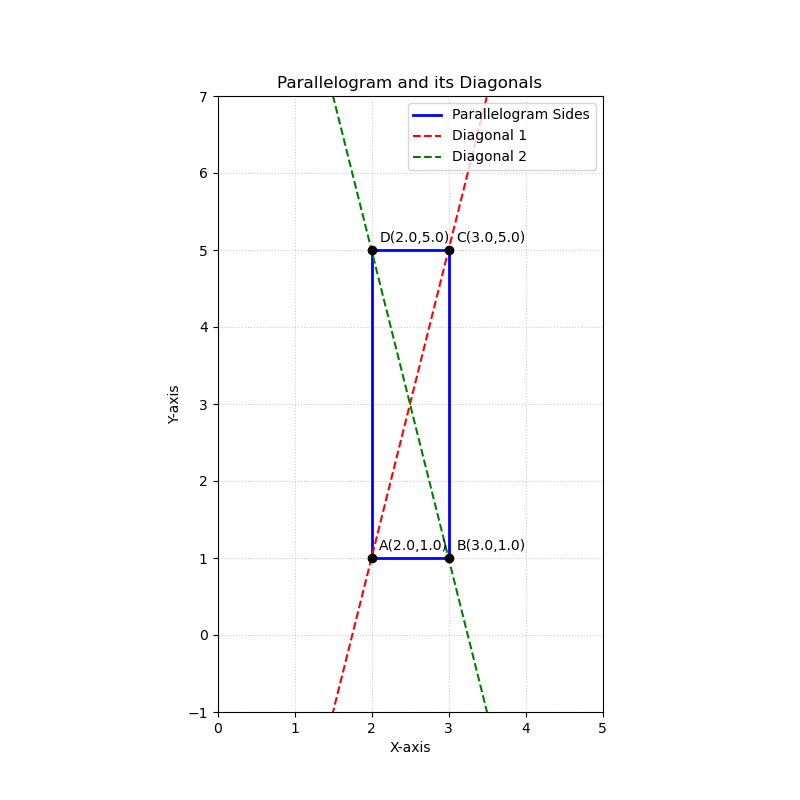
\includegraphics[width=\columnwidth, height=0.8\textheight, keepaspectratio]{figs/diagonals.png}     
\end{frame}

\begin{frame}[fragile]
    \frametitle{Python Code}
    \begin{lstlisting}
import numpy as np
import matplotlib.pyplot as plt

def solve_quadratic(a, b, c):
    discriminant = b**2 - 4*a*c
    if discriminant < 0:
        return None, None
    r1 = (-b + np.sqrt(discriminant)) / (2*a)
    r2 = (-b - np.sqrt(discriminant)) / (2*a)
    return r1, r2

def find_diagonals_python(x1, x2, y1, y2):
    A1 = y2 - y1
    B1 = x1 - x2
    C1 = (x2 * y1) - (x1 * y2)
    diag1_coeffs = [A1, B1, C1]
\end{lstlisting}
\end{frame}
\begin{frame}[fragile]
    \frametitle{Python Code}
    \begin{lstlisting}
    A2 = y1 - y2
    B2 = x1 - x2
    C2 = (x2 * y2) - (x1 * y1)
    diag2_coeffs = [A2, B2, C2]
    
    return diag1_coeffs, diag2_coeffs

def main():
    x1, x2 = solve_quadratic(1, -5, 6)
    y1, y2 = solve_quadratic(1, -6, 5)

    if x1 is None or y1 is None:
        print("Error: Could not solve quadratic equations. Check coefficients.")
        return
\end{lstlisting}
\end{frame}
\begin{frame}[fragile]
    \frametitle{Python Code}
    \begin{lstlisting}
    print(f"Parallelogram lines: x={x1}, x={x2}, y={y1}, y={y2}")

    d1, d2 = find_diagonals_python(x1, x2, y1, y2)
    
    print(f"Diagonal 1 (Ax+By+C=0): A={d1[0]:.1f}, B={d1[1]:.1f}, C={d1[2]:.1f}")
    print(f"Diagonal 2 (Ax+By+C=0): A={d2[0]:.1f}, B={d2[1]:.1f}, C={d2[2]:.1f}")

    fig, ax = plt.subplots(figsize=(8, 8))

    parallelogram_x = [x1, x2, x2, x1, x1]
    parallelogram_y = [y1, y1, y2, y2, y1]
    ax.plot(parallelogram_x, parallelogram_y, 'b-', label='Parallelogram Sides', linewidth=2)
\end{lstlisting}
\end{frame}
\begin{frame}[fragile]
    \frametitle{Python Code}
    \begin{lstlisting}
    plot_x_range = np.linspace(min(x1, x2) - 1, max(x1, x2) + 1, 100)
    
    def plot_line(coeffs, style, label):
        A, B, C = coeffs
        if abs(B) > 0:
            y_vals = (-A * plot_x_range - C) / B
            ax.plot(plot_x_range, y_vals, style, label=label)
        else:
            x_val = -C / A
            ax.axvline(x=x_val, linestyle=style.strip('-'), color=style[0], label=label)

    plot_line(d1, 'r--', 'Diagonal 1')
    plot_line(d2, 'g--', 'Diagonal 2')
\end{lstlisting}
\end{frame}
\begin{frame}[fragile]
    \frametitle{Python Code}
    \begin{lstlisting}
    ax.set_title('Parallelogram and its Diagonals')
    ax.set_xlabel('X-axis')
    ax.set_ylabel('Y-axis')
    ax.grid(True, linestyle=':', alpha=0.6)
    ax.legend()
    
    padding = 2
    ax.set_xlim(min(x1, x2) - padding, max(x1, x2) + padding)
    ax.set_ylim(min(y1, y2) - padding, max(y1, y2) + padding)
    ax.set_aspect('equal', adjustable='box')
\end{lstlisting}
\end{frame}
\begin{frame}[fragile]
    \frametitle{Python Code}
    \begin{lstlisting}
    x_min, x_max = min(x1, x2), max(x1, x2)
    y_min, y_max = min(y1, y2), max(y1, y2)
    vertices = {'A':(x_min, y_min), 'B':(x_max, y_min), 'C':(x_max, y_max), 'D':(x_min, y_max)}
    for name, (px, py) in vertices.items():
        ax.plot(px, py, 'ko')
        ax.text(px + 0.1, py + 0.1, f'{name}({px:.1f},{py:.1f})')
    plt.savefig("./figs/diagonals2.png") 
    plt.show()

if __name__ == "__main__":
    main()

\end{lstlisting}
\end{frame}


\begin{frame}{Plot-Using only Python}
    \centering
    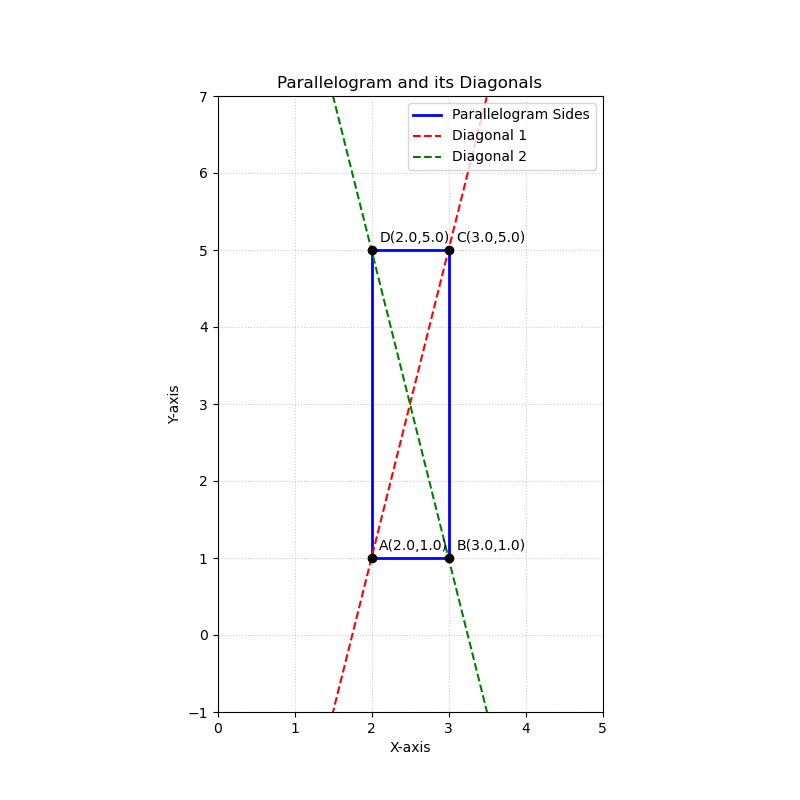
\includegraphics[width=\columnwidth, height=0.8\textheight, keepaspectratio]{figs/diagonals2.png}     
\end{frame}


\end{document}